\documentclass[9pt,landscape]{article}

\usepackage{multicol}
\usepackage{amsmath}
\usepackage{tabularx}

\usepackage{amssymb}
\usepackage{amsthm}
\usepackage{amsmath}
\usepackage{fontspec,xunicode,xltxtra}
\usepackage{titlesec}
\usepackage{indentfirst}
\usepackage{xeCJK}
\usepackage{fancyhdr}
\usepackage{graphicx}
\usepackage{listings}
\usepackage{printlen}
\usepackage{ifthen}
\usepackage[savepos]{zref}
\usepackage{multicol}
\usepackage{sectsty}
\usepackage{xcolor}
\usepackage[framemethod=tikz]{mdframed}
\usepackage{hyperref}

\usepackage[paper=a4paper]{geometry}
\geometry{headheight=2.6cm,headsep=3mm,footskip=13mm}
\geometry{top=2cm,bottom=2cm,left=2cm,right=2cm}


\setCJKmainfont[BoldFont={SimHei}]{SimSun}
\newfontfamily{\monotype}{Consolas}
%\newcommand{\monotype}{\tt}

\pagestyle{fancy}

\fancyhead[L]{MH3510 Regression Analysis}
%\fancyhead[C]{}
\fancyhead[R]{Pu Fanyi}

\setlength{\parindent}{0em}

% settings for listings
\lstset {
  basicstyle = \small\monotype,
  language = C++,
  tabsize = 2,
  breaklines = true,
  breakindent = 1.1em,
  numbers=right,
  stringstyle=\monotype,
  numberstyle=\footnotesize\ttfamily,
  firstnumber=last,
  basewidth={0.5em, 0.4em},
  frame=single
}

\usepackage{titlesec}

% Adjust spacing for section
\titlespacing*{\section}{0pt}{1ex plus 0.5ex minus .2ex}{1ex plus .2ex}

% Adjust spacing for subsection
\titlespacing*{\subsection}{0pt}{1ex plus 0.5ex minus .2ex}{1ex plus .2ex}

% Adjust spacing for subsubsection
\titlespacing*{\subsubsection}{0pt}{1ex plus 0.5ex minus .2ex}{1ex plus .2ex}

\usepackage{enumitem}
\setlist[enumerate]{itemsep=0pt, parsep=0pt, topsep=0pt}

% an amazing script
% converts an line-number to arbitrary string
\let\othelstnumber=\thelstnumber
\def\createlinenumber#1#2{
    \edef\thelstnumber{%
        \unexpanded{%
            \ifnum#1=\value{lstnumber}\relax
             \tt #2%
            \else}%
        \expandafter\unexpanded\expandafter{\thelstnumber\othelstnumber\fi}%
    }
    \ifx\othelstnumber=\relax\else
      \let\othelstnumber\relax
    \fi
}

\usepackage{enumitem}

\setlist[itemize]{itemsep=0pt}
 % formatting template

\begin{document}

\begin{multicols}{3}

\columnseprule=0.25pt

\section{公式}

$\mathrm{Var}(X)=\mathbb{E}(X^2)-(\mathbb{E}(X))^2$

$\Sigma_x = \mathbb{E}\left[(x-\mathbb{E}[x])(x-\mathbb{E}[x])^\top\right]$

$y=Ax\Rightarrow \Sigma_y=A\Sigma_xA^\top$

$A\perp\!\!\!\!\perp B\Rightarrow \sigma^2_{A\pm B}=\sigma^2_A + \sigma_B^2$

$X = \begin{bmatrix}
1&1&\cdots&1\\
x_1&x_2&\cdots&x_n
\end{bmatrix}^\top, X^\top X = \begin{bmatrix}
1&\sum x_i\\
\sum x_i&\sum x_i^2
\end{bmatrix}$

\section{Simple Linear Regression}

\subsection{Model Fitting}

Residual: $e_i=y_i-\hat{y}_i$

$y_i=\beta_0+\beta_1x_i+\epsilon_i, \mathbb{E}[\epsilon_i]=0, \mathrm{Var}(\epsilon_i)=\sigma^2$

$
\begin{cases}
S_{xx}=\sum_{i=1}^n\left(x_i-\overline{x}\right)^2\\
S_{xy}=\sum_{i=1}^{n}\left(x_i-\overline{x}\right)\left(y_i-\overline{y}\right)\\
S_{yy}=\sum_{i=1}^{n}\left(y_i-\overline{y}\right)^2
\end{cases}
$

$
\hat{\beta}_0=\overline{y}-\hat{\beta_1}\overline{x}, \hat{\beta}_1=\frac{S_{xy}}{S_{xx}}
$

Gauss-Markov Theorem (quality of LSE): Among all estimates that are linear combination of $y_1 , \cdots, y_n$ and unbiased, the LSE has the smallest variance.

$\sum_{i=1}^{n}e_i=0, \sum_{i=1}^{n}x_ie_i=0, \sum_{i=1}^{n}y_i=\sum_{i=1}^{n}\hat{y}_i$

\subsection{Statistic Inference \& Model Test}

Error sum of squares: $\mathrm{SSE}=\sum_{i=1}^{n}\left(y_i-\hat{y}_i\right)^2$

$s^2=\mathrm{MSE}=\frac{\mathrm{SSE}}{n-2}$

Regression sum of squares: $\mathrm{SSR}=\sum_{i=1}^{n}\left(\hat{y}_i-\overline{y}\right)^2$

$S_{yy}=\mathrm{SSR} + \mathrm{SSE}$

$\hat{\beta}_0=\boldsymbol{l}^\top\boldsymbol{y}, \hat{\beta}_1=\boldsymbol{k}^\top \boldsymbol{y}, k_i=\frac{x_i-\overline{x}}{S_{xx}}, l_i=\frac{1}{n}-k_i\overline{x}$

$\sum_{i=1}^{n}l_i=0, \sum_{i=1}^{n}l_ix_i=0$

$\frac{\hat{\beta}_1-\beta_1}{\sqrt{\sigma^2/S_{xx}}}\sim\mathcal{N}(0, 1), \frac{\hat{\beta}_0-\beta_0}{\sqrt{\left(\sigma^2\sum_{i=1}^{n}x_i^2\right)/\left(nS_{xx}\right)}}\sim\mathcal{N}(0, 1)$

$\frac{\hat{\beta}_1-\beta_1}{\sqrt{s^2/S_{xx}}}\sim t_{n-2}, \frac{\hat{\beta}_0-\beta_0}{\sqrt{\left(s^2\sum_{i=1}^{n}x_i^2\right)/\left(nS_{xx}\right)}}\sim t_{n-2}$

$
\frac{\hat{y}_0-\mathbb{E}[y_0]}{s\sqrt{\frac{1}{n}+\frac{\left(x_0-\overline{x}\right)^2}{S_{xx}}}}\sim t_{n-2}
$

$
\frac{y_{\text{new}}-\hat{y}_{\text{new}}}{s\sqrt{1+\frac{1}{n}+\frac{\left(x_0-\overline{x}\right)^2}{S_{xx}}}}\sim t_{n-2}
$

$
\mathcal{R}^2=\frac{\mathrm{SSR}}{S_{yy}}=\frac{S_{xy}^2}{S_{xx}S_{yy}}=r^2_{xy}
$

ANOVA for SLR:

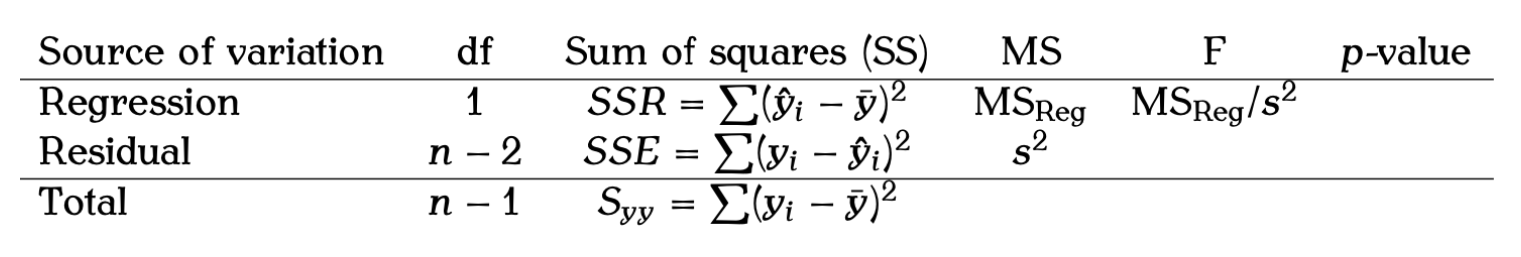
\includegraphics[width=\columnwidth]{imgs/ANOVA_for_SLR}

$\mathrm{MS}=\frac{\mathrm{SS}}{\mathrm{df}}$

$\mathrm{SSR}\sim \sigma^2\chi^2_1, \mathrm{SSE}\sim\sigma^2\chi^2_{n-2}$

$F=\frac{\mathrm{MS}_{\mathrm{reg}}}{s^2}\sim F(1, n-2)$

$\mathbb{E}[\mathrm{MS}_{\mathrm{reg}}]=\sigma^2+\beta_1^2S_{xx}$

$F$ 越大说明 $\mathrm{MS}_{\mathrm{reg}}$ 越大,也就是 $\mathrm{SSR}$ 的贡献更大,更能说明 $\beta_1\neq 0$, $X$ effective in explaining variation in $Y$

\subsection{Model Diagnostics}

Standardized (semistudentized) residual: $e_i^*=\frac{e_i}{\sqrt{\mathrm{MSE}}}$

Rule of Thumb: $\left|e_i^*\right|>3\Leftrightarrow\text{outliers}$

QQ-Plot: $k$-th smallest, $\sqrt{\mathrm{MSE}}\left[z\left(\frac{k-0.375}{0.25}\right)\right]$
\[
\begin{array}{|c|c|}
\hline
\text{residual} & \text{expected residual} \\
\hline
e_{\min} & \sqrt{\text{MSE}} \left[ z \left( \frac{1 - 0.375}{n + 0.25} \right) \right] \\
\hline
e_{\text{2nd smallest}} & \sqrt{\text{MSE}} \left[ z \left( \frac{2 - 0.375}{n + 0.25} \right) \right] \\
\hline
\vdots & \vdots \\
\hline
e_{\max} & \sqrt{\text{MSE}} \left[ z \left( \frac{n - 0.375}{n + 0.25} \right) \right] \\
\hline
\end{array}
\]

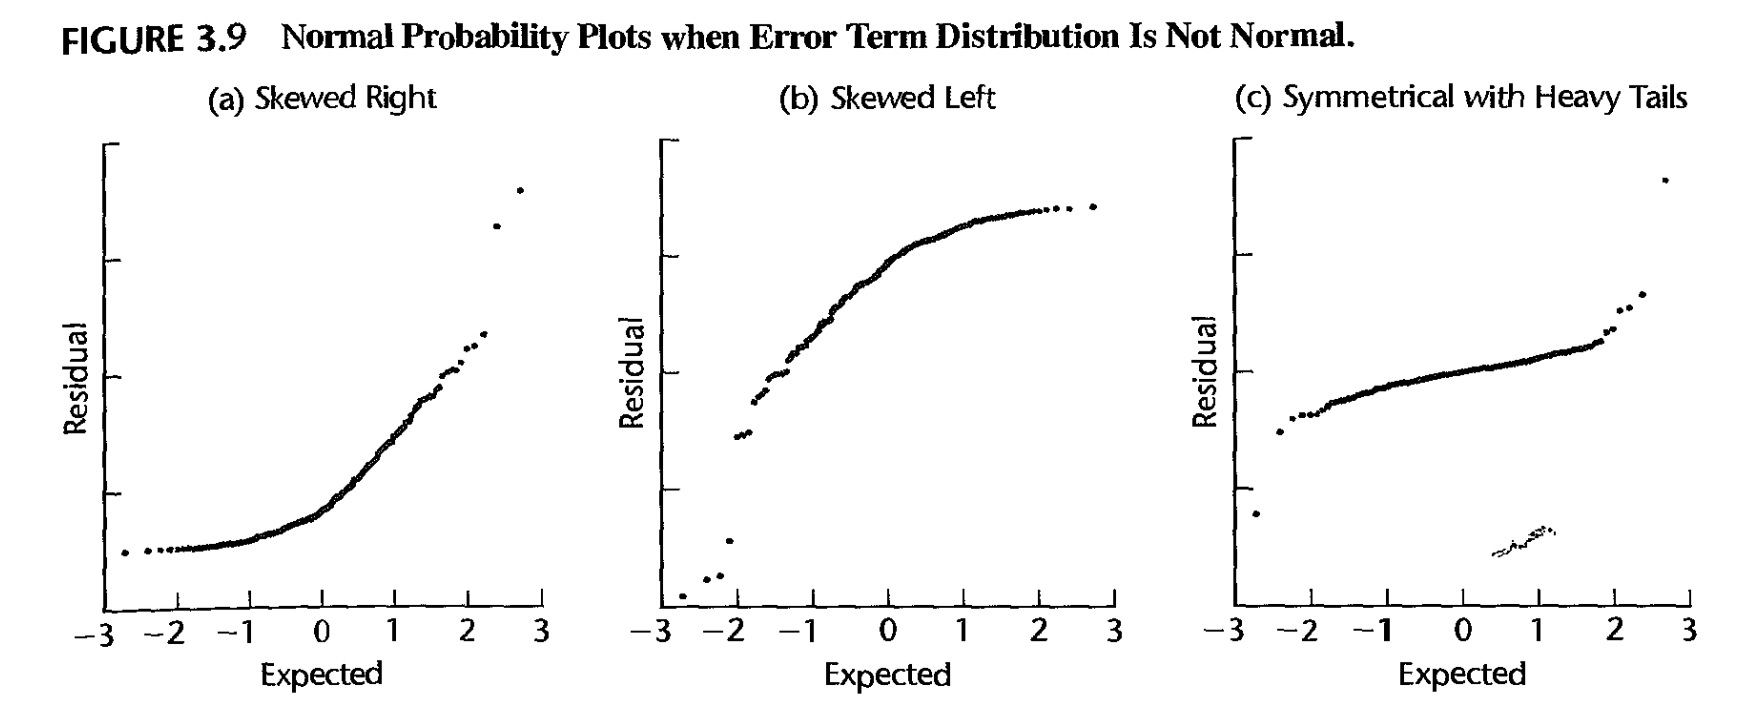
\includegraphics[width=\columnwidth]{imgs/qq-plot}

左边:往下尾巴大;
右边:往上尾巴大

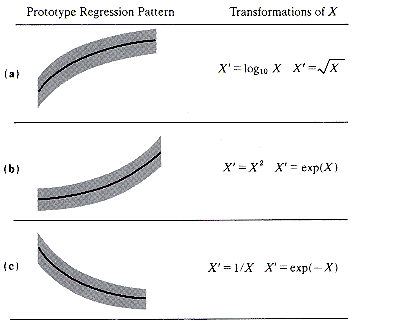
\includegraphics[width=\columnwidth]{imgs/trans1}

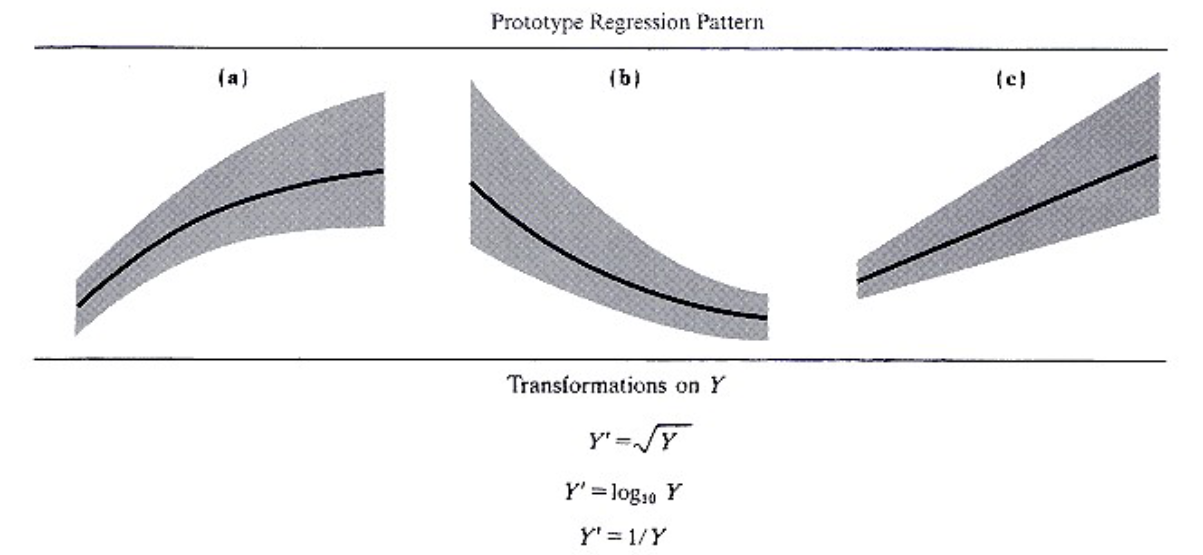
\includegraphics[width=\columnwidth]{imgs/trans2}

\section{Calculator}

$\mathtt{\sigma^2x}=\frac{1}{n}\sum_{i=1}^{n}(x_i-\overline{x})^2$

$\mathtt{s^2x}=\sqrt{\frac{1}{n-1}\sum_{i=1}^{n}(x_i-\overline{x})^2}$

$S_{xx}=n\cdot \mathtt{\sigma^2x}, S_{yy} = n\cdot \mathtt{\sigma^2y}$

$S_{xy} = \Sigma\mathtt{xy} - n\cdot\mathtt{\overline{x}}\cdot\mathtt{\overline{y}}$

\end{multicols}

\end{document}
